\section{METODOLOGI}

\subsection{Desain Robot yang Digunakan}

\begin{figure} [ht] \centering
	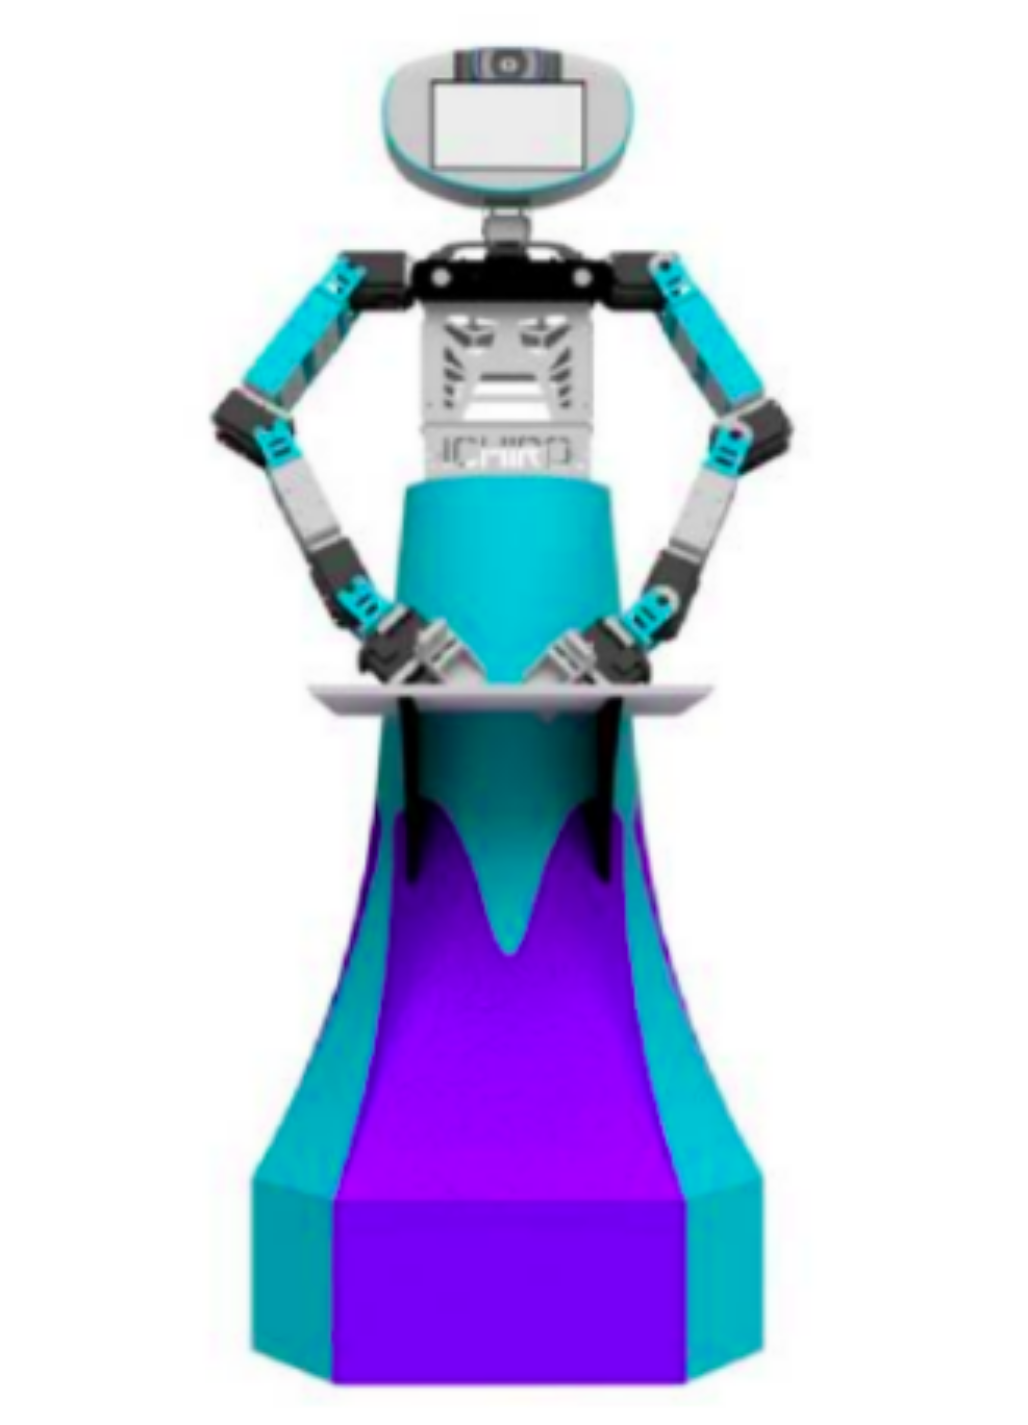
\includegraphics[scale=0.50]{gambar/robot-design.png}
	\caption{Desain robot yang digunakan}
	\label{fig:RobotDesign}
\end{figure}

Robot yang akan digunakan pada pada penelitian ini memiliki desain gabungan antara robot IRIS \citep{Dikairono2020} untuk setengah bagian bawahnya dan robot ICHIRO \citep{Muhtadin2019} untuk setengah bagian atasnya.
Desain ini secara umum dikenal sebagai \emph{mobile humanoid robot} \citep{Mohamed2012}, yang merupakan desain gabungan antara robot mobile dan robot humanoid.
Seperti yang terlihat pada Gambar \ref{fig:RobotDesign}, bagian bawah robot menyerupai robot mobile dengan \emph{omnidirectional wheels} yang memungkinkan pergerakan ke segala arah secara dua dimensi \citep{Oliveira2008}, sedangkan bagian atas robot menyerupai robot humanoid yang terdiri atas badan, kepala, dan lengan.
Dengan desain mobile humanoid robot ini, diharapkan pengguna bisa merasakan interaksi sosial yang lebih baik dengan robot karena memiliki bentuk mendekati manusia \citep{Rossi2018} sambil mempermudah navigasi dari robot ke berbagai tempat.

Robot ini dilengkapi dengan beberapa sensor seperti IMU (\emph{inertial measurement unit}) untuk mengetahui orientasi dari robot, Lidar untuk mendeteksi objek lain di sekitar robot, dan sensor kamera di kepala untuk menangkap citra yang nantinya bisa digunakan untuk mendeteksi objek menggunakan visi komputer.
Selain itu robot ini juga dilengkapi dengan dua lengan seperti robot manipulator yang bisa diatur pada berbagai posisi dan orientasi \citep{Iqbal2012}.
Dengan adanya sensor dan lengan ini diharapkan robot mampu melakukan tindakan \emph{assistive} secara sosial sesuai dengan data yang didapatkan dari sensor yang ada.

\subsection{Pembuatan Lingkungan Simulasi}

Lingkungan simulasi yang digunakan akan dibuat menggunakan simulator Gazebo.
Nantinya, lingkungan simulasi tersebut akan mensimulasikan suatu ruangan indoor yang terdiri atas berbagai macam objek.
Objek-objek yang ada di lingkungan simulasi tersebut secara umum akan terbagi menjadi dua jenis, yakni objek statis yang merepresentasikan benda yang tidak bisa bergerak sendiri seperti meja, kursi, dan lain sebagainya, serta objek dinamis yang merepresentasikan benda yang bisa bergerak secara bebas seperti robot dan pengguna.

Pada simulator Gazebo, sebuah lingkungan simulasi dengan berbagai macam objek yang ada di dalamnya dideskripsikan dalam bentuk \emph{Simulation Description Format} (SDF) \citep{SdfFormat}.
Agar bisa digunakan untuk membentuk suatu lingkungan simulasi, setiap objek yang ada akan dibuat menjadi sebuah file SDF yang nantinya bisa dengan mudah diletakkan dan digandakan di lingkungan simulasi, menyesuaikan dengan pengujian yang akan dilakukan.

Untuk objek robot, file SDF yang digunakan akan memiliki isi yang lebih lengkap dengan menyertakan kinematik pada robot mulai dari ujung bawah \emph{omnidirectional wheels} sampai bagian ujung lengan manipulator dan kepala, serta berbagai macam sensor virtual yang digunakan seperti IMU, Lidar, dan kamera.
Sedangkan untuk objek manusia akan menggunakan Actors yang merupakan model 3D dengan animasi yang bisa diprogram untuk bergerak dan berpose sesuai dengan keinginan \citep{GazeboActors}.

\subsection{Pengembangan Kontroler Robot}

\begin{figure} [ht] \centering
	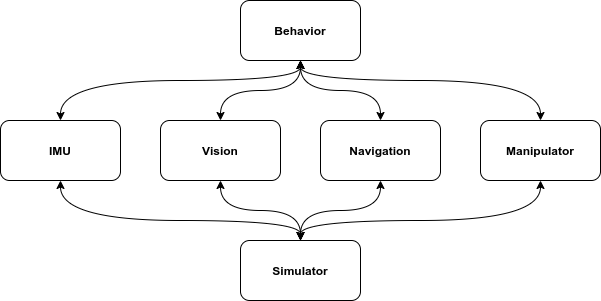
\includegraphics[scale=0.45]{gambar/robot-controller.png}
	\caption{Diagram sistem dari kontroler robot}
	\label{fig:RobotController}
\end{figure}

Kontroler robot yang digunakan untuk simulasi akan dikembangkan menggunakan ROS 2.
Kontroler tersebut akan terpisah menjadi beberapa node seperti yang terlihat pada Gambar \ref{fig:RobotController}.
Setiap node yang ada akan terhubung satu sama lain menggunakan sistem komunikasi antar proses ROS 2 yang berupa topics dan services.

Bagian utama dari kontroler robot tersebut adalah node Behavior yang berisi program yang mengatur segala tindakan robot berdasarkan data yang didapat dari sensor yang ada di simulasi.
Kemudian node Behavior tersebut akan terhubung dengan lima node lain yang merepresentasikan sensor dan aktuator yang ada pada robot.
Kelima node tersebut akan terpasang di dalam cakupan simulator Gazebo dalam bentuk plugins, sehingga mampu digunakan untuk mengakses dan memanipulasi data yang ada di simulasi menggunakan sistem \emph{shared memory} pada Gazebo \citep{GazeboPlugins}.

Sistem ini dirancang secara terpisah agar node Behavior yang diujikan di lingkungan simulasi bisa langsung bekerja pada robot fisik dengan cara mengubah keseluruhan cakupan yang ada di simulator Gazebo, termasuk kelima node yang telah disebutkan sebelumnya, menjadi node yang memproses sensor dan aktuator yang ada pada robot fisik.
Dengan ini pengujian yang dilakukan di simulasi bisa langsung diterapkan ketika diujikan pada robot fisik karena tidak perlunya pembuatan ulang kontroler yang menyesuaikan sistem yang ada pada robot.

\subsection{Pengujian Robot pada Lingkungan Simulasi}

Pengujian robot pada lingkungan simulasi akan dilakukan dengan cara menjalankan kontroler robot yang sudah dikembangkan dengan lingkungan simulasi yang sudah dibuat.
Pengujian tersebut akan dilakukan dalam dua cara yang berbeda.
Cara pertama akan menguji navigasi dari robot dengan cara memerintahkan robot untuk bergerak dari suatu titik ke titik yang lain, sedangkan cara kedua akan menguji visi komputer dari robot dengan cara mendeteksi objek pengguna yang terlihat di kamera dan kemudian mengubah posisi lengan dari robot tersebut jika ada objek pengguna yang terdeteksi.

Pengujian pertama akan dilakukan dengan cara menaruh robot di posisi acak yang ada di lingkungan simulasi, dan kemudian memerintahkannya untuk bergerak ke suatu titik yang juga dipilih secara acak.
Di dalam lingkungan simulasi tersebut, nantinya akan ada beberapa objek statis yang dapat menghalangi pergerakan dari robot.
Untuk mempermudah pengujian, navigasi akan dilakukan dengan bantuan beberapa package seperti Navigation 2 \citep{Navigation2} yang secara otomatis akan menentukan jalur navigasi dari robot dengan melihat orientasi dari sensor IMU dan objek penghalang di sekitar dari deteksi yang dilakukan oleh sensor Lidar.
Pengujian ini dilakukan dengan harapan untuk menguji apakah kedua sensor IMU dan Lidar serta pergerakan yang dimiliki robot dapat bekerja di simulasi.

Pengujian kedua akan dilakukan dengan cara menaruh robot di suatu tempat tanpa bergerak dan menunggu sampai ada objek pengguna yang terdeteksi di pandangan kamera robot.
Objek pengguna tersebut akan bergerak secara acak di sekitar robot, dan apabila ada objek pengguna yang terdeteksi oleh robot, maka robot akan mengubah posisi lengan manipulator ke atas.
Dalam pengujian ini, proses visi komputer akan dilakukan dengan bantuan TensorFlow \citep{TensorFlow} dan model yang sudah dilatih menggunakan COCO dataset \citep{CocoDataset}.
Pengujian ini dilakukan dengan harapan untuk menguji apakah sensor kamera dan aktuator lengan yang dimiliki robot dapat bekerja di simulasi.

\subsection{Pemindahan Kontroler ke Robot Fisik}

\begin{figure} [ht] \centering
	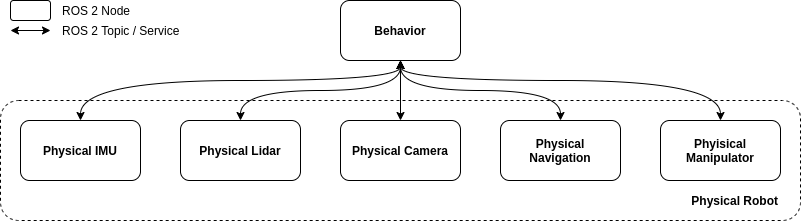
\includegraphics[scale=0.45]{gambar/controller-transfer.png}
	\caption{Diagram sistem dari kontroler robot untuk robot fisik.}
	\label{fig:ControllerTransfer}
\end{figure}

Untuk memastikan kontroler robot juga bisa bekerja di luar lingkungan simulasi, pengujian juga akan dilakukan pada robot fisik dengan cara menjalankan node Behavior yang sebelumnya digunakan di lingkungan simulasi.
Seperti yang terlihat pada Gambar \ref{fig:ControllerTransfer}, keseluruhan cakupan yang ada di simulator Gazebo akan digantikan dengan node-node lain yang memproses sensor dan aktuator yang ada pada robot fisik.
Node-node tersebut akan terhubung dengan node Behavior menggunakan komunikasi antar proses yang ada di ROS 2.
Untuk memastikan kontroler robot dapat bekerja dengan keseluruhan sensor dan aktuator yang ada di robot fisik, maka kedua cara pengujian yang dilakukan di lingkungan simulasi sebelumnya juga akan dilakukan pada robot fisik.
Percobaan pemindahan ini dilakukan untuk memastikan bahwa pengujian yang dilakukan di lingkungan simulasi dapat digunakan untuk menggantikan pengujian yang dilakukan menggunakan robot fisik.
